\documentclass[../../main.tex]{subfiles}

\begin{document}
\label{sec:abbildungen_graphen_intro}
\parpic[r]{
    \centering
    \begin{tikzpicture}[scale=.75]
    \draw[grayset] (-1.5,0) ellipse (0.7cm and 2cm);
    \draw[grayset] (1.5,0) ellipse (0.7cm and 2cm);

    \node (x1) at (-1.5,0.7) {$\bullet$};
    \node (x2) at (-1.5,-0.2) {$\bullet$};
    \node (x3) at (-1.5,-1.1) {$\bullet$};
    \node (y1) at (1.5,0.7) {$\bullet$};
    \node (y2) at (1.5,-0.2) {$\bullet$};
    \node (y3) at (1.5,-1.2) {$\bullet$};

    \draw[->] (x1) -- (y3);
    \draw[->] (x2) to[bend right] (y1);
    \draw[->] (x3) to[bend right] (y2);
\end{tikzpicture}%Also used by abbildungen/01einfuehrung
}

Zu Beginn des Kapitels haben wir bereits eine Möglichkeit gesehen, Abbildungen graphisch darzustellen. Da eine Abbildung eine Definitions- und eine Bildmenge hat, können wir diese beiden Mengen zeichnen und von jedem Argument einen Pfeil zu seinem Bild ziehen -- so wie im Bild rechts. 

Diese Darstellung ist anschaulich, hat aber einen großen Nachteil: Wenn die Definitionsmenge viele oder sogar unendlich viele Elemente hat (z.B. wenn eine Abbildung für alle natürlichen Zahlen, also \Natural, definiert ist), müssen wir selbst, wenn wir nur einen Ausschnitt zeichnen, sehr viele Pfeile zeichnen und es wird unübersichtlich.

Deshalb lernst du in diesem Abschnitt eine effektivere Methode, die Koordinatensysteme verwendet. Ein Punkt im Koordinatensystem hat eine $x$- und eine $y$-Koordinate. Während die $x$-Koordinate angibt, wie weit rechts oder links er ist, sagt die $y$-Koordinate aus, wie weit oben oder unten der Punkt ist. Wo ein Punkt liegt, wird also durch zwei Informationen beschrieben.

\begin{figure}[ht]
    \centering
    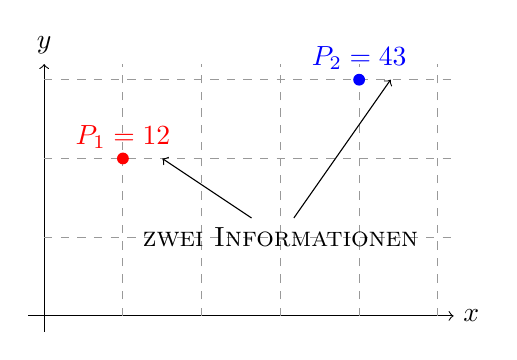
\begin{tikzpicture}
    \draw[->] (-0.2,0) -- (5.2,0) node[right] {$x$};
    \draw[->] (0,-0.2) -- (0,3.2) node[above] {$y$};
    \draw[dashed,black!40] (1,0) -- (1,3.2);
    \draw[dashed,black!40] (2,0) -- (2,3.2);
    \draw[dashed,black!40] (3,0) -- (3,3.2);
    \draw[dashed,black!40] (4,0) -- (4,3.2);
    \draw[dashed,black!40] (5,0) -- (5,3.2);
    \draw[dashed,black!40] (0,1) -- (5.2,1);
    \draw[dashed,black!40] (0,2) -- (5.2,2);
    \draw[dashed,black!40] (0,3) -- (5.2,3);
    
    \fill[red] (1,2) circle[radius=0.75mm] node[above] {$P_1=\coord{1}{2}$};
    \fill[blue] (4,3) circle[radius=0.75mm] node[above] {$P_2=\coord{4}{3}$};
    \node[align=center] (annotation) at (3,1) {\textsc{zwei Informationen}};
    \draw[->] (annotation) -- (4.4,3);
    \draw[->] (annotation) -- (1.5,2);
    \end{tikzpicture}
    \caption{Jeder der Punkte $P_1$ und $P_2$ benötigt zwei Informationen, um beschrieben zu werden. $P_1$ liegt bei $x$-Koordinate $1$ und $y$-Koordinate $2$. Würde eine dieser Informationen fehlen, wäre entweder nicht geklärt, wie weit rechts oder wie weit oben der Punkt liegt. Andersherum enthält die Position dieser Punkte natürlich auch genau diese zwei Informationen -- aus der Position von $P_2$ geht die $x$-Koordinate des Punktes ebenso wie die $y$-Koordinate hervor.}
\end{figure}

Wenn wir an die explizite Notation der Abbildungsvorschrift zurückdenken, dann hat jede Regel dort die Form $\text{Urbild}\mapsto\text{Bild}$. Sie enthält ebenfalls zwei Informationen -- erstens die Information über das Element der Definitionsmenge, das auf ein anderes abgebildet werden soll und zweitens die Information über das Bild dieses Elements.

Darauf aufbauend wollen wir die Koordinaten eines Punkts ab sofort nutzen, um eine Regel aus der Abbildungsvorschrift darzustellen. Jeder Punkt soll für ein bestimmtes Element der Definitionsmenge darstellen, wohin es abgebildet wird.

\begin{figure}[ht]
    \centering
    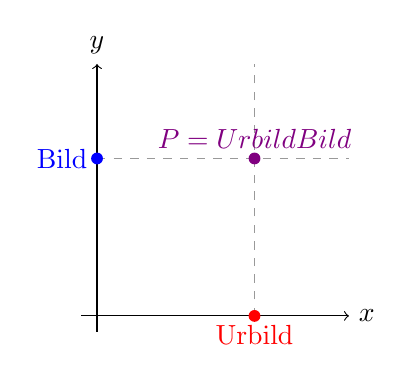
\begin{tikzpicture}
    \draw[->] (-0.2,0) -- (3.2,0) node[right] {$x$};
    \draw[->] (0,-0.2) -- (0,3.2) node[above] {$y$};
    \draw[dashed,black!40] (2,0) -- (2,3.2);
    \draw[dashed,black!40] (0,2) -- (3.2,2);
    
    \fill[red] (2,0) circle[radius=0.75mm] node[below] {Urbild};
    \fill[blue] (0,2) circle[radius=0.75mm] node[left] {Bild};
    \fill[violet] (2,2) circle[radius=0.75mm] node[above] {$P=\coord{\text{Urbild}}{\text{Bild}}$};
\end{tikzpicture}
    \caption{Jede Zuordnungsregel, die die Abbildungsvorschrift für ein bestimmtes Argument (Element der Definitionsmenge) festlegt, soll im Koordinatensystem durch einen einzelnen Punkt dargestellt werden.
    Im Bild ist zu sehen, wie die Position des entsprechenden Punktes von Urbild und Bild abhängt: Über jedem Element aus der Definitionsmenge ist genau ein Punkt abgebildet -- für das eindeutige Bild dieses Arguments. \emph{Wie weit} der Punkt über der $x$-Achse liegt, hängt davon ab, \emph{welches} Bild das Argument hat, das genauso weit rechts wie der eingezeichnete Punkt liegt.}
\end{figure}

Die Punkte, die eingezeichnet werden sollen, bekommen die Koordinate $P=(\text{Bild}|\text{Urbild})$. Nach wie vor soll der erste Wert angeben, wie weit rechts der Punkt im Koordinatensystem liegt -- und der zweite Wert, wie weit oben.
Über jedem möglichen Argument für die Abbildung ist also genau ein Punkt eingetragen, denn jedes Argument hat genau ein Bild  (und auf der Höhe, die dem Bild entspricht, ist dieser Punkt eingetragen).

Da an den Achsen eines normalen Koordinatensystems Zahlen stehen, Abbildungen aber beliebige Definitions- und Bildmengen haben können, ist erstmal unklar, wie Urbild-Bild-Paare angeben sollen, wie weit rechts oder links ein Punkt beispielsweise liegen muss. Die nächsten Abschnitte beschreiben, wie sich dieses Problem abhängig davon, welche Art von Definitionsmenge die Abbildung hat, lösen lässt.

\subsection{Abbildungen mit diskreten Definitionsmengen}
\label{sec:abbildungen_graphen_diskret}

Um Abbildungen im Koordinatensystem zu beschreiben, ist es zunächst einmal notwendig, die Definitions- und Bildmenge im Koordinatensystem zu repräsentieren. Dafür nutzt man die beiden Achsen des Koordinatensystems: Auf der $x$-Achse trägt man die Elemente der Definitionsmenge ein. Später wird man über jedem dieser Elemente genau einen Punkt einzeichnen. Die Höhe, in der man diesen Punkt einzeichnet, hängt vom Bild dieses Elements ab. Die Bildmenge zeichnet man also in die $y$-Achse -- dadurch legt man schließlich auch die Höhe der Punkte fest (denn jedes Bild ist nun einer Höhe auf der $y$-Achse zugeordnet). Nachdem die beiden Mengen eingezeichnet wurden, sieht das Koordinatensystem wie in der nächsten Abbildung aus.

\begin{figure}[ht]
    \centering
    \begin{tikzpicture}[scale=0.8]
        \draw[grayset] (0,1.75) ellipse (3mm and 1.75cm);
        \draw[grayset] (2.5,0) ellipse (25mm and 3mm);
        
        \draw[->] (-0.2,0) -- (5.1,0) node[right] {\textsc{Definitionsmenge}};
        \draw[->] (0,-0.2) -- (0,3.5) node[above] {\textsc{Bildmenge}};
        
        \fill (0,1) circle[radius=0.1];
        \fill (0,2) circle[radius=0.1];
        \fill (0,3) circle[radius=0.1];
        
        \fill (1.5,0) circle[radius=0.1];
        \fill (3,0) circle[radius=0.1];
        \fill (4.5,0) circle[radius=0.1];
    \end{tikzpicture}
    \caption{Dieses Bild zeigt, wie Definitions- und Bildmenge einer Abbildung ins Koordinatensystem eingezeichnet werden können. Die Definitionsmenge liegt quer, sodass die einzelnen Elemente davon auf der $x$-Achse untergebracht werden können. Die Bildmenge wird so eingezeichnet, dass sich ihre Elemente als Punkte auf der $y$-Achse einzeichnen lassen.}
\end{figure}

Es spielt erst einmal keine Rolle, in welcher Reihenfolge die Elemente eingezeichnet werden. Wichtig ist nur, dass sie alle auf der entsprechenden Koordinatenachse liegen. Mit diesem Schritt bereiten wir das Koordinatensystem vor, um im zweiten Schritt die Abbildungsvorschrift einzeichnen zu können.

\begin{example}{}
    \parpic[r]{
        \begin{tikzpicture}[scale=0.7]
            \draw[grayset] (0,1.75) ellipse (3mm and 1.75cm);
            \draw[grayset] (2.5,0) ellipse (25mm and 3mm);
            %
            \draw[->] (-0.2,0) -- (5.5,0);
            \draw[->] (0,-0.2) -- (0,3.8);
            %
            \node (D) at (3,1) {\textsc{Grundfarben}};
            \node (B) at (3,3) {\textsc{Mischfarben}};
            \draw[->] (D) -- (3.5,0.1);
            \draw[->] (B.west) to[bend right] (0.1,2.3);
            %
            \fill[yellow!70!black] (0,1) circle[radius=0.1] node[black, left] {gelb};
            \fill[orange] (0,2) circle[radius=0.1] node[black, left] {orange};
            \fill[green!70!black] (0,3) circle[radius=0.1] node[black, left] {grün};
            %
            \fill[yellow!70!black] (1.5,0) circle[radius=0.1] node[black, below] {gelb};
            \fill[red] (3,0) circle[radius=0.1] node[black, below] {rot};
            \fill[blue] (4.5,0) circle[radius=0.1] node[black, below] {blau};
        \end{tikzpicture}
    }
    \picskip{7}
    Nachdem das Koordinatensystem vorbereitet wurde, um die Abbildung \textsc{MitGelbMischen} im Koordinatensystem darzustellen, sieht es wie rechts abgebildet aus: Die Definitionsmenge von \textsc{MitGelbMischen} ist die Menge \textsc{Grundfarben}. Diese ist auf der $x$-Achse eingezeichnet.
    
    Die Bildmenge (die Menge \textsc{Mischfarben}) wird über die $y$-Achse gelegt. Damit kann jede Mischfarbe einen Punkt auf der $y$-Achse erhalten.
\end{example}

Jetzt ist es möglich, für jede Abbildungsregel der Form $\text{Urbild}\mapsto\text{Bild}$ den Punkt $\coord{\text{Urbild}}{\text{Bild}}$ einzuzeichnen. Dafür wird der Punkt in gerader Linie über dem Urbild eingezeichnet. Das Urbild wurde im vorherigen Schritt an einer Stelle auf der $x$-Achse platziert. Die Höhe des Punktes entspricht der Höhe, an der auf der $y$-Achse das Bildelement eingetragen wurde. Zeichnet man also vom Urbild eine Linie nach oben und vom Bild eine Linie nach rechts, dann stellt der Schnittpunkt die Abbildungsregel für diese beiden Elemente dar.

\begin{example}{}
    \parpic[r]{
        \begin{tikzpicture}[scale=0.8]
            \draw[->] (-0.2,0) -- (5.1,0) node[right,text width=2cm] {\textsc{Grund- farben}};
            \draw[->] (0,-0.2) -- (0,3.5) node[above] {\textsc{Mischfarben}};
            %
            \draw[dashed] (1.5,0) -- (1.5,1);
            \draw[dashed] (3,0) -- (3,2);
            \draw[dashed] (4.5,0) -- (4.5,3);
            \draw[dashed] (0,1) -- (1.5,1);
            \draw[dashed] (0,2) -- (3,2);
            \draw[dashed] (0,3) -- (4.5,3);
            %
            \fill[yellow!70!black] (0,1) circle[radius=0.1] node[black, left] {gelb};
            \fill[orange] (0,2) circle[radius=0.1] node[black, left] {orange};
            \fill[green!70!black] (0,3) circle[radius=0.1] node[black, left] {grün};
            %
            \fill[yellow!70!black] (1.5,0) circle[radius=0.1] node[black, below] {gelb};
            \fill[red] (3,0) circle[radius=0.1] node[black, below] {rot};
            \fill[blue] (4.5,0) circle[radius=0.1] node[black, below] {blau};
            %
            \fill (1.5,1) circle[radius=0.1] node[black, above] {$\text{gelb}\mapsto\text{gelb}$};
            \fill (3,2) circle[radius=0.1] node[black, above] {$\text{rot}\mapsto\text{orange}$};
            \fill (4.5,3) circle[radius=0.1] node[black, above] {$\text{blau}\mapsto\text{grün}$};
        \end{tikzpicture}
    }
    
    Im nebenstehenden Bild wurden die Abbildungsregeln durch die drei eingezeichneten schwarzen Punkte dargestellt. Der Punkt mit der Beschriftung $\text{blau}\mapsto\text{grün}$ liegt in gerader Linie über dem Urbild (blau) und in gerader Linie neben dem Bild (grün). So ist es möglich, am Punkt abzulesen, welche Regel er darstellt, auch wenn die Beschriftung nicht vorhanden wäre.
\end{example}

Durch das ungeordnete Eintragen der Definitions- und Bildmenge auf den Achsen hat man zunächst relativ wenig aus dem Koordinatensystem herausgeholt. Die Darstellung ist zunächst überhaupt nicht übersichtlicher. Das liegt daran, dass wir bisher nicht genutzt haben, dass sich bei Koordinatensystemen normalerweise eine Ordnung auf den Achsen befindet: Nach rechts bzw. oben werden die Werte immer größer.

Manche Definitions- und Bildmengen lassen es zu, dass wir ihre Elemente sinnvoll ordnen, etwa alphabetisch oder -- wenn es sich um Zahlen handelt -- nach der Größe.

Auf diese Weise kann es möglich sein, durch die Anordnung der Punkte durch kurzes Hinsehen sofort Informationen darüber zu erhalten, wie eine Abbildungsvorschrift aufgebaut ist. 

Gerade wenn man es mit Abbildungen zu tun hat, die nur mit Zahlen arbeiten, kann man einfach das gewohnte Koordinatensystem verwenden und für jede Zahl, die tatsächlich in der Definitionsmenge ist, einen Punkt auf der $x$-Achse eintragen (bzw. auf der $y$-Achse für Zahlen in der Bildmenge).

\begin{figure}[ht]
    \centering
    \begin{tikzpicture}[scale=0.7]
        \draw[->] (-0.2,0) -- (5.6,0) node[right] {$x$};
        \draw[->] (0,-0.2) -- (0,4.2) node[above] {$f(x)$};
        \foreach\y in {1,...,4}{
            \fill[blue] (0,\y) circle[radius=0.1] node[black, left] {$\y$};
        }
        \foreach\x in {0,...,5}{
            \fill[red] (\x,0) circle[radius=0.1] node[black, below] {$\x$};
        }
    \end{tikzpicture}
    \caption{Das Koordinatensystem, das hier zu sehen ist, eignet sich direkt, um Abbildungen darzustellen, die Zahlen auf Zahlen abbilden. Weil ohnehin jede Zahl einen Platz auf der $x$-Achse oder $y$-Achse hat, muss dort nicht noch zusätzlich eine Menge eingezeichnet werden.}
\end{figure}

\begin{example}{}
    \parpic[r]{
        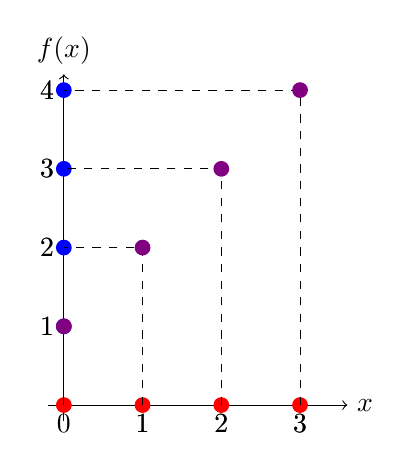
\begin{tikzpicture}
            \draw[->] (-0.2,0) -- (3.6,0) node[right] {$x$};
            \draw[->] (0,-0.2) -- (0,4.2) node[above] {$f(x)$};
            %
            \fill[blue] (0,1) circle[radius=0.1] node[black, left] {$1$};
            \fill[blue] (0,2) circle[radius=0.1] node[black, left] {$2$};
            \fill[blue] (0,3) circle[radius=0.1] node[black, left] {$3$};
            \fill[blue] (0,4) circle[radius=0.1] node[black, left] {$4$};
            %
            \fill[red] (0,0) circle[radius=0.1] node[black, below] {$0$};
            \fill[red] (1,0) circle[radius=0.1] node[black, below] {$1$};
            \fill[red] (2,0) circle[radius=0.1] node[black, below] {$2$};
            \fill[red] (3,0) circle[radius=0.1] node[black, below] {$3$};
            %
            \draw[dashed] (0,0) -- (0,1);
            \draw[dashed] (1,0) -- (1,2) -- (0,2);
            \draw[dashed] (2,0) -- (2,3) -- (0,3);
            \draw[dashed] (3,0) -- (3,4) -- (0,4);
            \draw[dashed] (0,0) -- (0,1) node[left]{$1$};
            \draw[dashed] (1,0) node[below]{$1$} -- (1,2) -- (0,2) node[left]{$2$};
            \draw[dashed] (2,0) node[below]{$2$} -- (2,3) -- (0,3) node[left]{$3$};
            \draw[dashed] (3,0) node[below]{$3$} -- (3,4) -- (0,4) node[left]{$4$};
            %
            \fill[violet] (0,1) circle[radius=0.1];
            \fill[violet] (1,2) circle[radius=0.1];
            \fill[violet] (2,3) circle[radius=0.1];
            \fill[violet] (3,4) circle[radius=0.1];
        \end{tikzpicture}
    }

    Im abgebildeten Koordinatensystem ist die Abbildung $f\colon\Natural\rightarrow\Natural$ zu sehen, die jede Zahl auf ihren Nachfolger abbildet. $f$ ist also durch die Berechnungsvorschrift $f(x)=x+1$ definiert.
    
    Die lilafarbenen Punkte, die zum Darstellen der Abbildungsvorschrift eingezeichnet wurden, sind in einem bestimtmen Muster angeordnet: Sie bilden eine nach oben führende Gerade. Diese Gerade würde natürlich auch nach rechts weitergehen, wenn ein größeres Koordinatensystem zur Verfügung stehen würde.
    
    \parpic[r]{1}
    Allein durch das kurze Betrachten des Bildes weißt du sofort etwas über die Abbildungsvorschrift (zum Beispiel, dass du größere Zahlen als Bilder du erhältst, je größer du das Argument wählst).
\end{example}

In den meisten mathematischen Anwendungen arbeitet man mit Abbildungen, die unendlich viele verschiedene Argumente erhalten können, also eine unendliche Definitionsmenge haben. Das ist zum Beispiel bei Abbildungen, deren Definitionsmenge die natürlichen Zahlen sind, der Fall. Deswegen stellen wir meistens nur einen bestimmten Ausschnitt der Abbildungsvorschrift dar.

Im letzten Bild endete die $x$-Achse beispielsweise bei der $3$. Das heißt, dass in diesem Koordinatensystem einfach alle Abbildungsregeln für Zahlen, die größer als $3$ sind, nicht mehr dargestellt werden. Das ist grundsätzlich kein Problem -- sondern sogar notwendig, da es ja nicht möglich ist, unendlich viele Punkte einzuzeichnen. Wenn man von einer Abbildung, die für alle natürliche Zahlen definiert ist, nur einen ausgewählten Bereich zeichnet, hat man automatisch wieder eine kleine, endliche Anzahl an Punkten übrig, die man einzeichnen muss.

Die Gesamtheit aller Punkte, die man zum Darstellen der Abbildungsvorschrift ins Koordinatensystem einzeichnet, nennt man den \textbf{Graph} der Abbildung. Im letzten Beispiel bestand der Graph von $f$ beispielsweise aus allen lilafarbenen Punkten.

\begin{definition}{Graph einer Abbildung}
        Für eine Abbildung $f\colon U\rightarrow V$ mit $U,V\subseteq \Real$ ist der \textbf{Graph} von $f$ die Menge aller Punkte im Koordinatensystem, deren Koordinate $\coord{x}{y}$ die Eigenschaft hat, dass $f(x)=y$ gilt. Der Graph von $f$ ist also die Menge $\{\coord{x}{y} \mid f(x)=y\}$.
\end{definition}

\subsection{Abbildungen mit dichten Definitionsmengen}
\label{sec:abbildungen_graphen_stetig}

Obwohl es nicht möglich ist, Abbildungen mit unendlicher Definitionsmenge vollständig graphisch darzustellen, gibt es eine gute Möglichkeit, sie trotzdem sinnvoll aufzuzeichnen. Im letzten Abschnitt hast du gesehen, dass du nur eine kleine Anzahl an Punkten zeichnen musst, wenn du nur ein Intervall aus der Definitionsmenge darstellst. 

Eine Abbildung $f\colon\Natural\rightarrow\Natural$ lässt sich beispielsweise zeichnen, indem du die Definitionsmenge nur bis zur Zahl $5$ (oder einer beliebigen anderen Zahl) darstellst. Dann besteht der Teil des Abbildungsgraphs, den du zeichnen musst, nur aus fünf Punkten. Dieser Trick funktioniert nicht bei einer bestimmten Art von Definitionsmengen, nämlich bei \textbf{dichten} Definitionsmengen. Das sind Mengen, bei denen in beliebig kleinen Bereichen schon beliebig viele Elemente auftauchen.

\begin{advanced}{Dichte Mengen}
    Eine Menge ist dicht, wenn sich zwischen zwei beliebigen Zahlen aus der Menge immer noch eine weitere Zahl finden lässt, die zwischen den beiden Zahlen liegt.
    
    \begin{definition}{Dichte Menge}
        Eine Menge $M$ heißt \textbf{dicht}, wenn für beliebige $m,m'\in M$ ein $x\in M$ existiert mit $m<x<m'$.
    \end{definition}
    
    \begin{advexample}{}
        Die Menge $\Rational$ ist dicht. Wählt man zum Beispiel die Zahlen $0$ und $1$, so liegt die Zahl $\frac{1}{2}$ zwischen diesen Zahlen. Egal wie klein man den Abstand zweier Zahlen wählt -- selbst, wenn man $0.0001$ und $0.0002$ wählt -- es gibt immer eine rationale Zahl zwischen den beiden Zahlen.
    \end{advexample}
\end{advanced}

Warum sind solche Definitionsmengen nun ein Problem? Wenn du einen Abbildungsgraphen für eine Abbildung mit dichter Definitionsmenge zeichnen möchtest, kannst du zwar links und rechts die Definitionsmenge abschneiden, indem du die Zeichnung dort aufhören lässt. Das Problem ist, dass trotzdem immer unendlich viele mögliche Argumente in deinem Bild auftauchen -- egal, wie weit du den Bereich einschränkst.

Nun sehen wir uns an, wie man das Zeichnen von unendlich vielen Punkten auch für Abbildungen vermeiden kann, deren Definitionsmenge dicht ist.

\begin{example}{}
    \begin{minipage}{\textwidth}
        Der Abbildungsgraph der Abbildung $f\colon\Real\rightarrow\Real$ mit $f(x)=1$ enthält die Punkte $\coord{0}{1}, \coord{1}{1}, \coord{2}{1}$ und $\coord{3}{1}$. Diese Punkte gehören in jedem Fall zum Graph von $f$. Sie können also sofort eingezeichnet werden. Man erhält eine Darstellung wie links.
        
        Anschließend fehlen weiterhin alle Punkte zwischen den eingezeichneten. Man kann also fortfahren, indem man auch einige davon einzeichnet -- und nächsten Schritt noch mehr. Schrittweise kommt man so zum mittleren bzw. rechten Bild.
        
        Macht man auf diese Weise immer weiter, dann haben die Punkte irgendwann keinen sichtbaren Abstand mehr und bilden letztlich einfach eine durchgezogene Linie.
        
        \begin{multicols}{3}
            \centering
            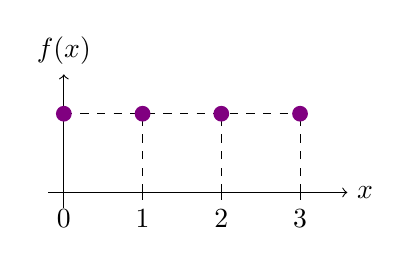
\begin{tikzpicture}
                \draw[->] (-0.2,0) -- (3.6,0) node[right] {$x$};
                \draw[->] (0,-0.2) -- (0,1.5) node[above] {$f(x)$};
                
                \draw[dashed] (0,1) -- (3,1);
                \foreach \x in {0,1,...,3}{
                    \draw (\x,0.1) -- (\x,-0.1) node[black, below] {$\x$};
                    \draw[dashed] (\x,0) -- (\x,1);
                    \fill[violet] (\x,1) circle[radius=0.1];
                }
            \end{tikzpicture}
            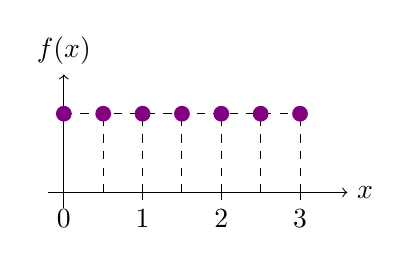
\begin{tikzpicture}
                \draw[->] (-0.2,0) -- (3.6,0) node[right] {$x$};
                \draw[->] (0,-0.2) -- (0,1.5) node[above] {$f(x)$};
                
                \draw[dashed] (0,1) -- (3,1);
                \foreach \x in {0,0.5,...,3}{
                    \draw[dashed] (\x,0) -- (\x,1);
                    \fill[violet] (\x,1) circle[radius=0.1];
                }
                \foreach \x in {0,1,...,3}{
                    \draw (\x,0.1) -- (\x,-0.1) node[black, below] {$\x$};
                }
            \end{tikzpicture}
            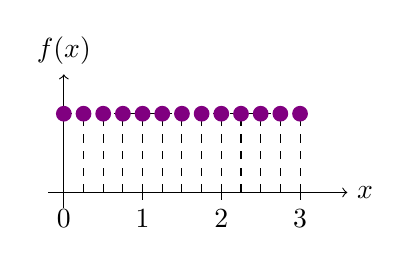
\begin{tikzpicture}
                \draw[->] (-0.2,0) -- (3.6,0) node[right] {$x$};
                \draw[->] (0,-0.2) -- (0,1.5) node[above] {$f(x)$};
                
                \draw[dashed] (0,1) -- (3,1);
                \foreach \x in {0,0.25,...,3}{
                    \draw[dashed] (\x,0) -- (\x,1);
                    \fill[violet] (\x,1) circle[radius=0.1];
                }
                \foreach \x in {0,1,...,3}{
                    \draw (\x,0.1) -- (\x,-0.1) node[black, below] {$\x$};
                }
            \end{tikzpicture}
        \end{multicols}
    \end{minipage}
\end{example}

Um den Graphen auch bei dichten Definitionsmengen zu zeichnen, kann man zunächst anfangen, indem man einige beliebige Punkte, die ins Bild passen, einzeichnet. Diese Punkte gehören auf jeden Fall zum Graphen. Zeichnet man nun einige weitere Punkte dazwischen, dann entwickelt sich der Graph wie im letzten Beispiel.

Aus einzelnen Punkten wird eine zusammenhängende Linie, weil es keinen freien Platz zwischen den einzelnen Punkten mehr gibt. Das passiert bei jeder dichten Definitionsmenge. Sobald du das vorher weißt, kannst du auch einfach direkt die Linie zeichnen, die du am Ende bekommen wirst. Es hilft aber dennoch, zunächst einzelne Punkte einzuzeichnen, damit du siehst, wie der Graph am Ende aussehen wird.

\begin{example}{}
    \parpic[r]{
        \begin{tikzpicture}
            \draw[->] (-0.2,0) -- (3.6,0) node[right] {$x$};
            \draw[->] (0,-0.2) -- (0,1.5) node[above] {$f(x)$};
            \foreach \x in {0,...,3}{
                \draw (\x,0.1) -- (\x,-0.1) node[black, below] {$\x$};
                \draw[dashed] (\x,0) -- (\x,1);
            }
            \draw[violet] (0,1) -- (3.3,1);
        \end{tikzpicture}
    }
    
    \picskip{7}
    Die Abbildung aus dem letzten Beispiel hat den rechts zu sehenden Graphen, der direkt als eine Linie gezeichnet wurde. Man kann es sich sparen, vorher einzelne Punkte einzuzeichnen, wenn man eine dichte Definitionsmenge hat, weil am Ende sowieso alle Punkte zu einer einzelnen Linie verschmelzen.
    
    Die eingezeichneten gestrichelten Linien sind hier nur Beispiele, bei welchen Argumenten man anfangen kann, einzelne Punkte auf dem Graphen zu finden, um zu sehen, wo die Linie entlangführt, die am Ende gezeichnet werden muss. Man hätte genauso gut an irgendeiner anderen Stelle ein Bild zu einem Argument berechnen und eine Linie zeichnen können. Grundsätzlich lässt man die gestrichelten Linien später einfach weg -- sie können aber dabei helfen, eine solche graphische Darstellung zu zeichnen.
\end{example}

Mithilfe des Koordinatensystems können wir nun Eigenschaften von Abbildungen \emph{sehen}. Für Abbildungen, die nicht so einfach sind, kann es später sehr hilfreich sein, sich mithilfe von Koordinatensystemen Informationen zu beschaffen, um sie besser zu verstehen.

Wir sind außerdem in der Lage, die Abbildungsregeln direkt im Koordinatensystem abzulesen. Dafür startet man auf der $x$-Achse bei einem beliebigen Wert und geht in gerader Linie nach oben, bis man den Graphen trifft. Auf der Höhe, auf der man auf den Graphen trifft, befindet sich auf der $y$-Achse auch das Bild, das wir suchen.

Auf ähnliche Weise können wir vorgehen, wenn wir die Urbilder zu einem Element der Bildmenge suchen -- wir fangen dann bei der $y$-Achse an und suchen den Graphen mit einer Linie nach links oder rechts (die man sich natürlich nur denkt statt sie wirklich einzuzeichnen). Allerdings muss man dann damit rechnen, dass man mehrere oder gar kein passendes Urbild findet (z.B. wenn die Abbildung das gewählte Bild niemals produziert).

\begin{example}{}
    \parpic[r]{
        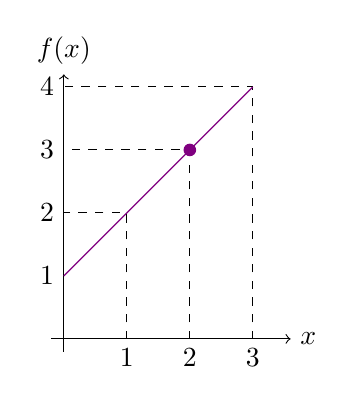
\begin{tikzpicture}[scale=0.8]
    \draw[->] (-0.2,0) -- (3.6,0) node[right] {$x$};
    \draw[->] (0,-0.2) -- (0,4.2) node[above] {$f(x)$};
    %
    \draw[dashed] (0,0) -- (0,1) node[left]{$1$};
    \draw[dashed] (1,0) node[below]{$1$} -- (1,2) -- (0,2) node[left]{$2$};
    \draw[dashed] (2,0) node[below]{$2$} -- (2,3) -- (0,3) node[left]{$3$};
    \draw[dashed] (3,0) node[below]{$3$} -- (3,4) -- (0,4) node[left]{$4$};
    %
    \draw[violet] (0,1) -- (3,4);
    \fill[violet] (2,3) circle[radius=1mm];
\end{tikzpicture}%Also used by abbildunge/06_eigenschaften_von_abbildungen
    }
    
    Am rechts abgebildeten Abbildungsgraph können die Bilder von beliebigen Elementen der Definitionsmenge abgelesen werden. Um beispielsweise abzulesen, auf welche Zahl das Argument $2$ abgebildet wird, beginnst du dort, wo die Zahl $2$ auf der $x$-Achse eingetragen ist und schaust dann auf einer geraden Linie nach oben, wo du den Graph triffst.
    
    In diesem Fall triffst du den Graphen beim eingezeichneten lilafarbenen Punkt. Um nun herauszufinden, welchem Element der Bildmenge der getroffene Punkt entspricht, verfolgst du vom eingezeichneten Punkt eine gerade Linie nach links, bis du die $y$-Achse triffst. Vom lila eingezeichneten Punkt kommst du zur $3$. Dies ist das Bild, das wir gesucht haben. Es gilt also $f(2)=3$.
    
    Auf die gleiche Weise kann mit den entsprechenden eingezeichneten gestrichtelten Linien auch z.B. das Bild von der $1$ oder $3$ gefunden werden.
\end{example}

\begin{nutshell}{Abbildungen in Koordinatensystemen darstellen}
    \parpic[r]{
        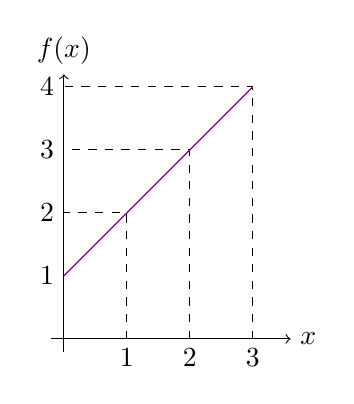
\begin{tikzpicture}[scale=0.8]
            \draw[->] (-0.2,0) -- (3.6,0) node[right] {$x$};
            \draw[->] (0,-0.2) -- (0,4.2) node[above] {$f(x)$};
            %
            \draw[dashed] (0,0) -- (0,1) node[left]{$1$};
            \draw[dashed] (1,0) node[below]{$1$} -- (1,2) -- (0,2) node[left]{$2$};
            \draw[dashed] (2,0) node[below]{$2$} -- (2,3) -- (0,3) node[left]{$3$};
            \draw[dashed] (3,0) node[below]{$3$} -- (3,4) -- (0,4) node[left]{$4$};
            %
            \draw[violet] (0,1) -- (3,4);
        \end{tikzpicture}
    }
    
    Die Darstellung von Abbildungen mit Mengendiagrammen ist bei großen Definitionsmengen sehr unpraktisch und die Pfeile stellen die Abbildungsvorschrift nicht übersichtlich dar.
    
    Deswegen stellt man Abbildungen normalerweise im Koordinatensystem dar, indem man einen \textbf{Abbildungsgraph} einzeichnet. Dafür stellt die $x$-Achse die Elemente der Definitionsmenge und die $y$-Achse die Elemente der Bildmenge dar. Über jedem $x$-Wert wird ein Punkt auf der Höhe seines Bildes eingezeichnet. 
    
    Ist die Definitionsmenge \textbf{dicht}, dann verbindet man die eingezeichneten Punkte zu einer durchgehenden Linie, um den \textbf{Graph} der Abbildung zu erhalten.
\end{nutshell}

\end{document}